% Options for packages loaded elsewhere
\PassOptionsToPackage{unicode}{hyperref}
\PassOptionsToPackage{hyphens}{url}
%
\documentclass[
]{article}
\usepackage{amsmath,amssymb}
\usepackage{iftex}
\ifPDFTeX
  \usepackage[T1]{fontenc}
  \usepackage[utf8]{inputenc}
  \usepackage{textcomp} % provide euro and other symbols
\else % if luatex or xetex
  \usepackage{unicode-math} % this also loads fontspec
  \defaultfontfeatures{Scale=MatchLowercase}
  \defaultfontfeatures[\rmfamily]{Ligatures=TeX,Scale=1}
\fi
\usepackage{lmodern}
\ifPDFTeX\else
  % xetex/luatex font selection
\fi
% Use upquote if available, for straight quotes in verbatim environments
\IfFileExists{upquote.sty}{\usepackage{upquote}}{}
\IfFileExists{microtype.sty}{% use microtype if available
  \usepackage[]{microtype}
  \UseMicrotypeSet[protrusion]{basicmath} % disable protrusion for tt fonts
}{}
\makeatletter
\@ifundefined{KOMAClassName}{% if non-KOMA class
  \IfFileExists{parskip.sty}{%
    \usepackage{parskip}
  }{% else
    \setlength{\parindent}{0pt}
    \setlength{\parskip}{6pt plus 2pt minus 1pt}}
}{% if KOMA class
  \KOMAoptions{parskip=half}}
\makeatother
\usepackage{xcolor}
\usepackage[margin=1in]{geometry}
\usepackage{color}
\usepackage{fancyvrb}
\newcommand{\VerbBar}{|}
\newcommand{\VERB}{\Verb[commandchars=\\\{\}]}
\DefineVerbatimEnvironment{Highlighting}{Verbatim}{commandchars=\\\{\}}
% Add ',fontsize=\small' for more characters per line
\usepackage{framed}
\definecolor{shadecolor}{RGB}{248,248,248}
\newenvironment{Shaded}{\begin{snugshade}}{\end{snugshade}}
\newcommand{\AlertTok}[1]{\textcolor[rgb]{0.94,0.16,0.16}{#1}}
\newcommand{\AnnotationTok}[1]{\textcolor[rgb]{0.56,0.35,0.01}{\textbf{\textit{#1}}}}
\newcommand{\AttributeTok}[1]{\textcolor[rgb]{0.13,0.29,0.53}{#1}}
\newcommand{\BaseNTok}[1]{\textcolor[rgb]{0.00,0.00,0.81}{#1}}
\newcommand{\BuiltInTok}[1]{#1}
\newcommand{\CharTok}[1]{\textcolor[rgb]{0.31,0.60,0.02}{#1}}
\newcommand{\CommentTok}[1]{\textcolor[rgb]{0.56,0.35,0.01}{\textit{#1}}}
\newcommand{\CommentVarTok}[1]{\textcolor[rgb]{0.56,0.35,0.01}{\textbf{\textit{#1}}}}
\newcommand{\ConstantTok}[1]{\textcolor[rgb]{0.56,0.35,0.01}{#1}}
\newcommand{\ControlFlowTok}[1]{\textcolor[rgb]{0.13,0.29,0.53}{\textbf{#1}}}
\newcommand{\DataTypeTok}[1]{\textcolor[rgb]{0.13,0.29,0.53}{#1}}
\newcommand{\DecValTok}[1]{\textcolor[rgb]{0.00,0.00,0.81}{#1}}
\newcommand{\DocumentationTok}[1]{\textcolor[rgb]{0.56,0.35,0.01}{\textbf{\textit{#1}}}}
\newcommand{\ErrorTok}[1]{\textcolor[rgb]{0.64,0.00,0.00}{\textbf{#1}}}
\newcommand{\ExtensionTok}[1]{#1}
\newcommand{\FloatTok}[1]{\textcolor[rgb]{0.00,0.00,0.81}{#1}}
\newcommand{\FunctionTok}[1]{\textcolor[rgb]{0.13,0.29,0.53}{\textbf{#1}}}
\newcommand{\ImportTok}[1]{#1}
\newcommand{\InformationTok}[1]{\textcolor[rgb]{0.56,0.35,0.01}{\textbf{\textit{#1}}}}
\newcommand{\KeywordTok}[1]{\textcolor[rgb]{0.13,0.29,0.53}{\textbf{#1}}}
\newcommand{\NormalTok}[1]{#1}
\newcommand{\OperatorTok}[1]{\textcolor[rgb]{0.81,0.36,0.00}{\textbf{#1}}}
\newcommand{\OtherTok}[1]{\textcolor[rgb]{0.56,0.35,0.01}{#1}}
\newcommand{\PreprocessorTok}[1]{\textcolor[rgb]{0.56,0.35,0.01}{\textit{#1}}}
\newcommand{\RegionMarkerTok}[1]{#1}
\newcommand{\SpecialCharTok}[1]{\textcolor[rgb]{0.81,0.36,0.00}{\textbf{#1}}}
\newcommand{\SpecialStringTok}[1]{\textcolor[rgb]{0.31,0.60,0.02}{#1}}
\newcommand{\StringTok}[1]{\textcolor[rgb]{0.31,0.60,0.02}{#1}}
\newcommand{\VariableTok}[1]{\textcolor[rgb]{0.00,0.00,0.00}{#1}}
\newcommand{\VerbatimStringTok}[1]{\textcolor[rgb]{0.31,0.60,0.02}{#1}}
\newcommand{\WarningTok}[1]{\textcolor[rgb]{0.56,0.35,0.01}{\textbf{\textit{#1}}}}
\usepackage{longtable,booktabs,array}
\usepackage{calc} % for calculating minipage widths
% Correct order of tables after \paragraph or \subparagraph
\usepackage{etoolbox}
\makeatletter
\patchcmd\longtable{\par}{\if@noskipsec\mbox{}\fi\par}{}{}
\makeatother
% Allow footnotes in longtable head/foot
\IfFileExists{footnotehyper.sty}{\usepackage{footnotehyper}}{\usepackage{footnote}}
\makesavenoteenv{longtable}
\usepackage{graphicx}
\makeatletter
\def\maxwidth{\ifdim\Gin@nat@width>\linewidth\linewidth\else\Gin@nat@width\fi}
\def\maxheight{\ifdim\Gin@nat@height>\textheight\textheight\else\Gin@nat@height\fi}
\makeatother
% Scale images if necessary, so that they will not overflow the page
% margins by default, and it is still possible to overwrite the defaults
% using explicit options in \includegraphics[width, height, ...]{}
\setkeys{Gin}{width=\maxwidth,height=\maxheight,keepaspectratio}
% Set default figure placement to htbp
\makeatletter
\def\fps@figure{htbp}
\makeatother
\setlength{\emergencystretch}{3em} % prevent overfull lines
\providecommand{\tightlist}{%
  \setlength{\itemsep}{0pt}\setlength{\parskip}{0pt}}
\setcounter{secnumdepth}{-\maxdimen} % remove section numbering
\usepackage{booktabs}
\usepackage{longtable}
\usepackage{array}
\usepackage{multirow}
\usepackage{wrapfig}
\usepackage{float}
\usepackage{colortbl}
\usepackage{pdflscape}
\usepackage{tabu}
\usepackage{threeparttable}
\usepackage{threeparttablex}
\usepackage[normalem]{ulem}
\usepackage{makecell}
\usepackage{xcolor}
\ifLuaTeX
  \usepackage{selnolig}  % disable illegal ligatures
\fi
\usepackage{bookmark}
\IfFileExists{xurl.sty}{\usepackage{xurl}}{} % add URL line breaks if available
\urlstyle{same}
\hypersetup{
  pdftitle={Motor Trend Data Regression Analysis},
  pdfauthor={Aadil Panjvani},
  hidelinks,
  pdfcreator={LaTeX via pandoc}}

\title{Motor Trend Data Regression Analysis}
\author{Aadil Panjvani}
\date{2024-11-06}

\begin{document}
\maketitle

\section{Executive Summary}\label{executive-summary}

This analysis was done for Motor Trend, a magazine about the automobile
industry. The task was to look at the mtcars data set of a collection of
cars. They are interested in exploring the relationship between a set of
variables and miles per gallon (MPG) (outcome).

They are particularly interested in the following two questions:

\begin{itemize}
\tightlist
\item
  ``Is an automatic or manual transmission better for MPG''
\item
  ``Quantify the MPG difference between automatic and manual
  transmissions''
\end{itemize}

After concluding the analysis, the following points can be made:

\begin{itemize}
\tightlist
\item
  Manual transmission y for MPG, based on the evidence from the box
  plot, as well as the simple linear regression model.
\item
  With a 95\% confidence interval, we estimate the true difference
  between automatic and manual cars to be between 3.2 and 11.3
\item
  Our simple linear model with transmission type as predictor shows us
  that the manual transmission cars have 7.24 (+/- 3.60) MPG more in
  fuel efficiency than automatic cars.
\item
  As for a multivariate linear regression model, using a stepwise
  selection method, we found that the predictor variables wt, qsec and
  am best predict mpg, explaining roughly 85\% of it's variation. This
  model was further tested with anova, the variance inflation factor,
  along with residual diagnostic plots.
\item
  This multivariate regression model tells us that, while adjusting for
  the other predictor variables wt and qsec, manual transmission cars on
  average have 2.94 MPG (+/- 2.89) more in fuel efficiency than
  automatic cars.
\end{itemize}

\section{Importing libraries}\label{importing-libraries}

\begin{Shaded}
\begin{Highlighting}[]
\FunctionTok{library}\NormalTok{(GGally)}
\FunctionTok{library}\NormalTok{(dplyr)}
\FunctionTok{library}\NormalTok{(ggplot2)}
\FunctionTok{library}\NormalTok{(car)}
\FunctionTok{library}\NormalTok{(broom)}
\FunctionTok{library}\NormalTok{(printr)}
\FunctionTok{library}\NormalTok{(pander)}
\FunctionTok{library}\NormalTok{(kableExtra)}

\FunctionTok{theme\_set}\NormalTok{(}\FunctionTok{theme\_classic}\NormalTok{())}
\end{Highlighting}
\end{Shaded}

\section{Exploring Data Analysis}\label{exploring-data-analysis}

To know more about the data, you can look at the appendix section with
title `About the data'

\begin{Shaded}
\begin{Highlighting}[]
\FunctionTok{head}\NormalTok{(mtcars) }\SpecialCharTok{\%\textgreater{}\%} \FunctionTok{kbl}\NormalTok{() }\SpecialCharTok{\%\textgreater{}\%} \FunctionTok{kable\_styling}\NormalTok{(}\AttributeTok{bootstrap\_options =} \FunctionTok{c}\NormalTok{(}\StringTok{"striped"}\NormalTok{, }\StringTok{"hover"}\NormalTok{))}
\end{Highlighting}
\end{Shaded}

\begin{table}
\centering
\begin{tabular}[t]{l|r|r|r|r|r|r|r|r|r|r|r}
\hline
  & mpg & cyl & disp & hp & drat & wt & qsec & vs & am & gear & carb\\
\hline
Mazda RX4 & 21.0 & 6 & 160 & 110 & 3.90 & 2.620 & 16.46 & 0 & 1 & 4 & 4\\
\hline
Mazda RX4 Wag & 21.0 & 6 & 160 & 110 & 3.90 & 2.875 & 17.02 & 0 & 1 & 4 & 4\\
\hline
Datsun 710 & 22.8 & 4 & 108 & 93 & 3.85 & 2.320 & 18.61 & 1 & 1 & 4 & 1\\
\hline
Hornet 4 Drive & 21.4 & 6 & 258 & 110 & 3.08 & 3.215 & 19.44 & 1 & 0 & 3 & 1\\
\hline
Hornet Sportabout & 18.7 & 8 & 360 & 175 & 3.15 & 3.440 & 17.02 & 0 & 0 & 3 & 2\\
\hline
Valiant & 18.1 & 6 & 225 & 105 & 2.76 & 3.460 & 20.22 & 1 & 0 & 3 & 1\\
\hline
\end{tabular}
\end{table}

Since vs and am are factor variables, we'll be factorizing them to get
more interpretable outputs in regression.

The question focuses on the am variable, which is transmission type -
automatic or manual. To answer the question, we can plot a box plot to
see the difference between automatic and manual.

Based on the box plot in the appendix, we can form a hypothesis that the
manual cars have higher miles per gallon, which means it has higher fuel
efficiency as compared to automatic cars. o test for this claim, we can
use a statistical test such as the t test.

\section{Two sample t test}\label{two-sample-t-test}

\begin{Shaded}
\begin{Highlighting}[]
\FunctionTok{panderOptions}\NormalTok{(}\StringTok{\textquotesingle{}table.split.table\textquotesingle{}}\NormalTok{, }\StringTok{\textquotesingle{}50\textquotesingle{}}\NormalTok{)}
\FunctionTok{pander}\NormalTok{(}\FunctionTok{t.test}\NormalTok{(mtcars}\SpecialCharTok{$}\NormalTok{mpg }\SpecialCharTok{\textasciitilde{}}\NormalTok{ mtcars}\SpecialCharTok{$}\NormalTok{am))}
\end{Highlighting}
\end{Shaded}

\begin{longtable}[]{@{}
  >{\centering\arraybackslash}p{(\columnwidth - 10\tabcolsep) * \real{0.1491}}
  >{\centering\arraybackslash}p{(\columnwidth - 10\tabcolsep) * \real{0.0702}}
  >{\centering\arraybackslash}p{(\columnwidth - 10\tabcolsep) * \real{0.1316}}
  >{\centering\arraybackslash}p{(\columnwidth - 10\tabcolsep) * \real{0.2193}}
  >{\centering\arraybackslash}p{(\columnwidth - 10\tabcolsep) * \real{0.2281}}
  >{\centering\arraybackslash}p{(\columnwidth - 10\tabcolsep) * \real{0.2018}}@{}}
\caption{Welch Two Sample t-test: \texttt{mtcars\$mpg} by
\texttt{mtcars\$am}}\tabularnewline
\toprule\noalign{}
\begin{minipage}[b]{\linewidth}\centering
Test statistic
\end{minipage} & \begin{minipage}[b]{\linewidth}\centering
df
\end{minipage} & \begin{minipage}[b]{\linewidth}\centering
P value
\end{minipage} & \begin{minipage}[b]{\linewidth}\centering
Alternative hypothesis
\end{minipage} & \begin{minipage}[b]{\linewidth}\centering
mean in group automatic
\end{minipage} & \begin{minipage}[b]{\linewidth}\centering
mean in group manual
\end{minipage} \\
\midrule\noalign{}
\endfirsthead
\toprule\noalign{}
\begin{minipage}[b]{\linewidth}\centering
Test statistic
\end{minipage} & \begin{minipage}[b]{\linewidth}\centering
df
\end{minipage} & \begin{minipage}[b]{\linewidth}\centering
P value
\end{minipage} & \begin{minipage}[b]{\linewidth}\centering
Alternative hypothesis
\end{minipage} & \begin{minipage}[b]{\linewidth}\centering
mean in group automatic
\end{minipage} & \begin{minipage}[b]{\linewidth}\centering
mean in group manual
\end{minipage} \\
\midrule\noalign{}
\endhead
\bottomrule\noalign{}
\endlastfoot
-3.767 & 18.33 & 0.001374 * * & two.sided & 17.15 & 24.39 \\
\end{longtable}

From the t test, we get a significant p-value, this means we can reject
the null that there is no difference between auto and manual cars. In
other words, the probability that the difference in these two groups
appeared by chance is very low. Observing the confidence interval, we
are 95\% confident that the true difference between automatic and manual
cars are between 3.2 and 11.3.

Since we'll be fitting regression models on this data, it's useful to
look pairwise scatter plots as this gives us a quick look into the
relationship between variables. This plot can be observed at the
appendix.

\section{Regression Model and Hypothesis
testing}\label{regression-model-and-hypothesis-testing}

\subsection{Simple Linear Regression
Model}\label{simple-linear-regression-model}

Since Motor Trends is more interested in the am variable, we'll be
fitting it to the model and observe the results.

\begin{Shaded}
\begin{Highlighting}[]
\NormalTok{fit\_am }\OtherTok{\textless{}{-}} \FunctionTok{lm}\NormalTok{(mpg }\SpecialCharTok{\textasciitilde{}}\NormalTok{ am, mtcars)}
\FunctionTok{summary}\NormalTok{(fit\_am) }
\end{Highlighting}
\end{Shaded}

\begin{verbatim}
## 
## Call:
## lm(formula = mpg ~ am, data = mtcars)
## 
## Residuals:
##     Min      1Q  Median      3Q     Max 
## -9.3923 -3.0923 -0.2974  3.2439  9.5077 
## 
## Coefficients:
##             Estimate Std. Error t value Pr(>|t|)    
## (Intercept)   17.147      1.125  15.247 1.13e-15 ***
## ammanual       7.245      1.764   4.106 0.000285 ***
## ---
## Signif. codes:  0 '***' 0.001 '**' 0.01 '*' 0.05 '.' 0.1 ' ' 1
## 
## Residual standard error: 4.902 on 30 degrees of freedom
## Multiple R-squared:  0.3598, Adjusted R-squared:  0.3385 
## F-statistic: 16.86 on 1 and 30 DF,  p-value: 0.000285
\end{verbatim}

The reference variable follows an alphabetical order, so interpreting
the coefficients, note that the reference variable in this case is
automatic transmission.

\begin{itemize}
\tightlist
\item
  The intercept here shows us that 17.15 is mean mpg for automatic
  transmission.
\item
  The slope coefficient shows us that 7.24 is the change in mean between
  the automatic and manual transmission (this can be observed from the
  box plot previously)
\item
  The p-value for the slope coefficient tells us that the mean
  difference between auto and manual transmission is significant, and
  thus we can conclude that manual transmission is more fuel efficient
  as compared to automatic.
\item
  The r squared for our model is low, with only 36\% of variation
  explained by the model. This makes sense because models with only one
  variable usually isn't enough.
\end{itemize}

Simple linear regression is usually insufficient in terms of creating a
good model that can predict mpg because there are other predictor
variables or regressors that can help explain more variation in the
model. Thus, this is where multivariate linear regression can help us
fit more variables to produce a better model.

\subsection{Multivariate Linear Regression
Model}\label{multivariate-linear-regression-model}

The goal is to create a model that best predicts mpg, or ultimately fuel
efficiency. This means that each of the predictors variables should have
a statistically significant p-value and are not correlated in any way
(this will be tested with the Variance Inflation factor later on). Model
fit can also be tested with anova, where you can observe whether adding
a variable explains away a significant portion of variation (or looking
at the p-value).

The challenge with Multivariate regression is which variables you should
include or remove. Here we see what happens if we include all the
variables in the data.

\begin{Shaded}
\begin{Highlighting}[]
\NormalTok{full.model }\OtherTok{\textless{}{-}} \FunctionTok{lm}\NormalTok{(mpg }\SpecialCharTok{\textasciitilde{}}\NormalTok{ ., }\AttributeTok{data =}\NormalTok{ mtcars)}
\FunctionTok{summary}\NormalTok{(full.model) }
\end{Highlighting}
\end{Shaded}

\begin{verbatim}
## 
## Call:
## lm(formula = mpg ~ ., data = mtcars)
## 
## Residuals:
##     Min      1Q  Median      3Q     Max 
## -3.4506 -1.6044 -0.1196  1.2193  4.6271 
## 
## Coefficients:
##             Estimate Std. Error t value Pr(>|t|)  
## (Intercept) 12.30337   18.71788   0.657   0.5181  
## cyl         -0.11144    1.04502  -0.107   0.9161  
## disp         0.01334    0.01786   0.747   0.4635  
## hp          -0.02148    0.02177  -0.987   0.3350  
## drat         0.78711    1.63537   0.481   0.6353  
## wt          -3.71530    1.89441  -1.961   0.0633 .
## qsec         0.82104    0.73084   1.123   0.2739  
## vs1          0.31776    2.10451   0.151   0.8814  
## ammanual     2.52023    2.05665   1.225   0.2340  
## gear         0.65541    1.49326   0.439   0.6652  
## carb        -0.19942    0.82875  -0.241   0.8122  
## ---
## Signif. codes:  0 '***' 0.001 '**' 0.01 '*' 0.05 '.' 0.1 ' ' 1
## 
## Residual standard error: 2.65 on 21 degrees of freedom
## Multiple R-squared:  0.869,  Adjusted R-squared:  0.8066 
## F-statistic: 13.93 on 10 and 21 DF,  p-value: 3.793e-07
\end{verbatim}

You can see that almost all (besides wt) the variables have p-values
that are not significant

An issue with multivariate regression is certain variables may be
correlated with each other, which can increase the standard error of
other variables. To assess colinearity, we can use the Variance
inflation factor, which r has a nifty function (vif) that does so.

\begin{Shaded}
\begin{Highlighting}[]
\FunctionTok{rbind}\NormalTok{(}\FunctionTok{vif}\NormalTok{(full.model))  }\SpecialCharTok{\%\textgreater{}\%}
  \FunctionTok{kbl}\NormalTok{() }\SpecialCharTok{\%\textgreater{}\%}
  \FunctionTok{kable\_styling}\NormalTok{(}\AttributeTok{bootstrap\_options =} \FunctionTok{c}\NormalTok{(}\StringTok{"striped"}\NormalTok{, }\StringTok{"hover"}\NormalTok{))}
\end{Highlighting}
\end{Shaded}

\begin{table}
\centering
\begin{tabular}[t]{r|r|r|r|r|r|r|r|r|r}
\hline
cyl & disp & hp & drat & wt & qsec & vs & am & gear & carb\\
\hline
15.37383 & 21.62024 & 9.832037 & 3.37462 & 15.16489 & 7.527958 & 4.965873 & 4.648487 & 5.357452 & 7.908747\\
\hline
\end{tabular}
\end{table}

We see some of the variables have really high VIF (more than 10) which
shows signs of co linearity.

\subsection{Stepwise regression model}\label{stepwise-regression-model}

There are many ways to test for different variables to choose the best
model, here I will be using the stepwise selection method to help find
the predictor variables that can best explain MPG.

\begin{Shaded}
\begin{Highlighting}[]
\NormalTok{bestModel }\OtherTok{\textless{}{-}} \FunctionTok{step}\NormalTok{(full.model, }\AttributeTok{direction =} \StringTok{"both"}\NormalTok{,}
                  \AttributeTok{trace =} \ConstantTok{FALSE}\NormalTok{)}
\FunctionTok{summary}\NormalTok{(bestModel)}
\end{Highlighting}
\end{Shaded}

\begin{verbatim}
## 
## Call:
## lm(formula = mpg ~ wt + qsec + am, data = mtcars)
## 
## Residuals:
##     Min      1Q  Median      3Q     Max 
## -3.4811 -1.5555 -0.7257  1.4110  4.6610 
## 
## Coefficients:
##             Estimate Std. Error t value Pr(>|t|)    
## (Intercept)   9.6178     6.9596   1.382 0.177915    
## wt           -3.9165     0.7112  -5.507 6.95e-06 ***
## qsec          1.2259     0.2887   4.247 0.000216 ***
## ammanual      2.9358     1.4109   2.081 0.046716 *  
## ---
## Signif. codes:  0 '***' 0.001 '**' 0.01 '*' 0.05 '.' 0.1 ' ' 1
## 
## Residual standard error: 2.459 on 28 degrees of freedom
## Multiple R-squared:  0.8497, Adjusted R-squared:  0.8336 
## F-statistic: 52.75 on 3 and 28 DF,  p-value: 1.21e-11
\end{verbatim}

Using the stepwise method, we end up with 3 predictor variables, wt,
qsec and am.

\begin{itemize}
\tightlist
\item
  all three variables have significant p-values, which suggest that they
  are all important addition to the model for predicting mpg.
\item
  note that our am variable has a less significant p-value after
  adjusting for variabes wt and qsec
\item
  after adjusting for other predictor variables, our coefficient for am
  went down to 2.94, and our pvalue became less significant.
\item
  The r squared value denotes how much of the variation in mpg is
  explained. Our best model explains around 84\% of the variation, which
  indicates it's a good model.
\end{itemize}

\section{Regression Diagnostics}\label{regression-diagnostics}

\begin{Shaded}
\begin{Highlighting}[]
\NormalTok{vif }\OtherTok{\textless{}{-}} \FunctionTok{cbind}\NormalTok{(}\FunctionTok{vif}\NormalTok{(bestModel))}
\FunctionTok{colnames}\NormalTok{(vif) }\OtherTok{\textless{}{-}} \StringTok{"VIF of bestmodel"}
\NormalTok{vif  }\SpecialCharTok{\%\textgreater{}\%}
  \FunctionTok{kbl}\NormalTok{() }\SpecialCharTok{\%\textgreater{}\%}
  \FunctionTok{kable\_styling}\NormalTok{(}\AttributeTok{bootstrap\_options =} \FunctionTok{c}\NormalTok{(}\StringTok{"striped"}\NormalTok{, }\StringTok{"hover"}\NormalTok{), }\AttributeTok{full\_width =}\NormalTok{ F)}
\end{Highlighting}
\end{Shaded}

\begin{table}
\centering
\begin{tabular}[t]{l|r}
\hline
  & VIF of bestmodel\\
\hline
wt & 2.482951\\
\hline
qsec & 1.364339\\
\hline
am & 2.541437\\
\hline
\end{tabular}
\end{table}

The variance inflation factor of all three of our variables are small,
which means they are not highly correlated.

\#\#Anova test on nested models

Anova is a useful statistical tool to use on nested models. With it, we
can interpret what the effects of adding a new variable are on the
coefficients and the p-values

\begin{Shaded}
\begin{Highlighting}[]
\NormalTok{fit0 }\OtherTok{\textless{}{-}} \FunctionTok{lm}\NormalTok{(mpg }\SpecialCharTok{\textasciitilde{}}\NormalTok{ am, mtcars)}
\NormalTok{fit1 }\OtherTok{\textless{}{-}} \FunctionTok{update}\NormalTok{(fit0, mpg }\SpecialCharTok{\textasciitilde{}}\NormalTok{ am }\SpecialCharTok{+}\NormalTok{ wt)}
\NormalTok{fit2 }\OtherTok{\textless{}{-}} \FunctionTok{update}\NormalTok{(fit1, mpg }\SpecialCharTok{\textasciitilde{}}\NormalTok{ am }\SpecialCharTok{+}\NormalTok{ wt }\SpecialCharTok{+}\NormalTok{ qsec)}
\NormalTok{fit3 }\OtherTok{\textless{}{-}} \FunctionTok{update}\NormalTok{(fit2, mpg }\SpecialCharTok{\textasciitilde{}}\NormalTok{ am }\SpecialCharTok{+}\NormalTok{ wt }\SpecialCharTok{+}\NormalTok{ qsec }\SpecialCharTok{+}\NormalTok{ disp)}
\NormalTok{fit4 }\OtherTok{\textless{}{-}} \FunctionTok{update}\NormalTok{(fit3, mpg }\SpecialCharTok{\textasciitilde{}}\NormalTok{ am }\SpecialCharTok{+}\NormalTok{ wt }\SpecialCharTok{+}\NormalTok{ qsec }\SpecialCharTok{+}\NormalTok{ disp }\SpecialCharTok{+}\NormalTok{ hp)}

\FunctionTok{anova}\NormalTok{(fit0, fit1, fit2, fit3, fit4)  }\SpecialCharTok{\%\textgreater{}\%}
  \FunctionTok{kbl}\NormalTok{() }\SpecialCharTok{\%\textgreater{}\%}
  \FunctionTok{kable\_styling}\NormalTok{(}\AttributeTok{bootstrap\_options =} \FunctionTok{c}\NormalTok{(}\StringTok{"striped"}\NormalTok{, }\StringTok{"hover"}\NormalTok{))}
\end{Highlighting}
\end{Shaded}

\begin{table}
\centering
\begin{tabular}[t]{r|r|r|r|r|r}
\hline
Res.Df & RSS & Df & Sum of Sq & F & Pr(>F)\\
\hline
30 & 720.8966 & NA & NA & NA & NA\\
\hline
29 & 278.3197 & 1 & 442.57690 & 74.9945513 & 0.0000000\\
\hline
28 & 169.2859 & 1 & 109.03377 & 18.4757461 & 0.0002140\\
\hline
27 & 166.0099 & 1 & 3.27607 & 0.5551293 & 0.4629119\\
\hline
26 & 153.4378 & 1 & 12.57205 & 2.1303314 & 0.1563873\\
\hline
\end{tabular}
\end{table}

Looking at the results, we see how our best fit gives us a significant
result (consistent with our stepwise selection model), but adding the
variables disp and hp gives us p-values that are not significant, thus a
worse model.

\subsection{Residual diganostic plots}\label{residual-diganostic-plots}

To diagnose a regression model it's also important to look at the
residual diagnostics, which can be seen at the appendix.

\begin{itemize}
\tightlist
\item
  From our residual vs fitted plot, we don't see any distinct patterns,
  which is a good sign
\item
  Our normal Q-Q plot shows that our standardized residuals are
  considerably normal, and doesn't deviate that much from the line.
\item
  scale-location is compares standardized residuals with fitted values,
  and we don't see any patterns as well
\item
  Our residual vs leverage plot don't contain any systematic patterns.
\end{itemize}

\#Appendix

\#\#Code

\begin{Shaded}
\begin{Highlighting}[]
\FunctionTok{library}\NormalTok{(GGally)}
\FunctionTok{library}\NormalTok{(dplyr)}
\FunctionTok{library}\NormalTok{(ggplot2)}
\FunctionTok{library}\NormalTok{(car)}
\FunctionTok{library}\NormalTok{(broom)}
\FunctionTok{library}\NormalTok{(printr)}
\FunctionTok{library}\NormalTok{(pander)}
\FunctionTok{library}\NormalTok{(kableExtra)}

\FunctionTok{theme\_set}\NormalTok{(}\FunctionTok{theme\_classic}\NormalTok{())}
\end{Highlighting}
\end{Shaded}

\begin{Shaded}
\begin{Highlighting}[]
\FunctionTok{head}\NormalTok{(mtcars) }\SpecialCharTok{\%\textgreater{}\%}
  \FunctionTok{kbl}\NormalTok{() }\SpecialCharTok{\%\textgreater{}\%}
  \FunctionTok{kable\_styling}\NormalTok{(}\AttributeTok{bootstrap\_options =} \FunctionTok{c}\NormalTok{(}\StringTok{"striped"}\NormalTok{, }\StringTok{"hover"}\NormalTok{))}
\end{Highlighting}
\end{Shaded}

\begin{Shaded}
\begin{Highlighting}[]
\CommentTok{\# factoring categorical variables for regression}
\NormalTok{mtcars }\OtherTok{\textless{}{-}}\NormalTok{ mtcars }\SpecialCharTok{\%\textgreater{}\%}
    \FunctionTok{mutate}\NormalTok{(}\AttributeTok{am =} \FunctionTok{factor}\NormalTok{(am, }\AttributeTok{labels =} \FunctionTok{c}\NormalTok{(}\StringTok{"automatic"}\NormalTok{, }\StringTok{"manual"}\NormalTok{))) }\SpecialCharTok{\%\textgreater{}\%}
    \FunctionTok{mutate}\NormalTok{(}\AttributeTok{vs =} \FunctionTok{factor}\NormalTok{(vs))}
\end{Highlighting}
\end{Shaded}

\begin{Shaded}
\begin{Highlighting}[]
\FunctionTok{panderOptions}\NormalTok{(}\StringTok{\textquotesingle{}table.split.table\textquotesingle{}}\NormalTok{, }\StringTok{\textquotesingle{}50\textquotesingle{}}\NormalTok{)}
\FunctionTok{pander}\NormalTok{(}\FunctionTok{t.test}\NormalTok{(mtcars}\SpecialCharTok{$}\NormalTok{mpg }\SpecialCharTok{\textasciitilde{}}\NormalTok{ mtcars}\SpecialCharTok{$}\NormalTok{am))}
\end{Highlighting}
\end{Shaded}

\begin{Shaded}
\begin{Highlighting}[]
\NormalTok{fit\_am }\OtherTok{\textless{}{-}} \FunctionTok{lm}\NormalTok{(mpg }\SpecialCharTok{\textasciitilde{}}\NormalTok{ am, mtcars)}
\FunctionTok{summary}\NormalTok{(fit\_am) }
\end{Highlighting}
\end{Shaded}

\begin{Shaded}
\begin{Highlighting}[]
\NormalTok{full.model }\OtherTok{\textless{}{-}} \FunctionTok{lm}\NormalTok{(mpg }\SpecialCharTok{\textasciitilde{}}\NormalTok{ ., }\AttributeTok{data =}\NormalTok{ mtcars)}
\FunctionTok{summary}\NormalTok{(full.model) }
\end{Highlighting}
\end{Shaded}

\begin{Shaded}
\begin{Highlighting}[]
\FunctionTok{rbind}\NormalTok{(}\FunctionTok{vif}\NormalTok{(full.model))  }\SpecialCharTok{\%\textgreater{}\%}
  \FunctionTok{kbl}\NormalTok{() }\SpecialCharTok{\%\textgreater{}\%}
  \FunctionTok{kable\_styling}\NormalTok{(}\AttributeTok{bootstrap\_options =} \FunctionTok{c}\NormalTok{(}\StringTok{"striped"}\NormalTok{, }\StringTok{"hover"}\NormalTok{))}
\end{Highlighting}
\end{Shaded}

\begin{Shaded}
\begin{Highlighting}[]
\NormalTok{bestModel }\OtherTok{\textless{}{-}} \FunctionTok{step}\NormalTok{(full.model, }\AttributeTok{direction =} \StringTok{"both"}\NormalTok{,}
                  \AttributeTok{trace =} \ConstantTok{FALSE}\NormalTok{)}
\FunctionTok{summary}\NormalTok{(bestModel)}
\end{Highlighting}
\end{Shaded}

\begin{Shaded}
\begin{Highlighting}[]
\NormalTok{vif }\OtherTok{\textless{}{-}} \FunctionTok{cbind}\NormalTok{(}\FunctionTok{vif}\NormalTok{(bestModel))}
\FunctionTok{colnames}\NormalTok{(vif) }\OtherTok{\textless{}{-}} \StringTok{"VIF of bestmodel"}
\NormalTok{vif  }\SpecialCharTok{\%\textgreater{}\%}
  \FunctionTok{kbl}\NormalTok{() }\SpecialCharTok{\%\textgreater{}\%}
  \FunctionTok{kable\_styling}\NormalTok{(}\AttributeTok{bootstrap\_options =} \FunctionTok{c}\NormalTok{(}\StringTok{"striped"}\NormalTok{, }\StringTok{"hover"}\NormalTok{), }\AttributeTok{full\_width =}\NormalTok{ F)}
\end{Highlighting}
\end{Shaded}

\begin{Shaded}
\begin{Highlighting}[]
\NormalTok{fit0 }\OtherTok{\textless{}{-}} \FunctionTok{lm}\NormalTok{(mpg }\SpecialCharTok{\textasciitilde{}}\NormalTok{ am, mtcars)}
\NormalTok{fit1 }\OtherTok{\textless{}{-}} \FunctionTok{update}\NormalTok{(fit0, mpg }\SpecialCharTok{\textasciitilde{}}\NormalTok{ am }\SpecialCharTok{+}\NormalTok{ wt)}
\NormalTok{fit2 }\OtherTok{\textless{}{-}} \FunctionTok{update}\NormalTok{(fit1, mpg }\SpecialCharTok{\textasciitilde{}}\NormalTok{ am }\SpecialCharTok{+}\NormalTok{ wt }\SpecialCharTok{+}\NormalTok{ qsec)}
\NormalTok{fit3 }\OtherTok{\textless{}{-}} \FunctionTok{update}\NormalTok{(fit2, mpg }\SpecialCharTok{\textasciitilde{}}\NormalTok{ am }\SpecialCharTok{+}\NormalTok{ wt }\SpecialCharTok{+}\NormalTok{ qsec }\SpecialCharTok{+}\NormalTok{ disp)}
\NormalTok{fit4 }\OtherTok{\textless{}{-}} \FunctionTok{update}\NormalTok{(fit3, mpg }\SpecialCharTok{\textasciitilde{}}\NormalTok{ am }\SpecialCharTok{+}\NormalTok{ wt }\SpecialCharTok{+}\NormalTok{ qsec }\SpecialCharTok{+}\NormalTok{ disp }\SpecialCharTok{+}\NormalTok{ hp)}

\FunctionTok{anova}\NormalTok{(fit0, fit1, fit2, fit3, fit4)  }\SpecialCharTok{\%\textgreater{}\%}
  \FunctionTok{kbl}\NormalTok{() }\SpecialCharTok{\%\textgreater{}\%}
  \FunctionTok{kable\_styling}\NormalTok{(}\AttributeTok{bootstrap\_options =} \FunctionTok{c}\NormalTok{(}\StringTok{"striped"}\NormalTok{, }\StringTok{"hover"}\NormalTok{))}
\end{Highlighting}
\end{Shaded}

\subsection{About the data}\label{about-the-data}

A data frame with 32 observations on 11 (numeric) variables.

{[}, 1{]} mpg Miles/(US) gallon {[}, 2{]} cyl Number of cylinders {[},
3{]} disp Displacement (cu.in.) {[}, 4{]} hp Gross horsepower {[}, 5{]}
drat Rear axle ratio {[}, 6{]} wt Weight (1000 lbs) {[}, 7{]} qsec 1/4
mile time {[}, 8{]} vs Engine (0 = V-shaped, 1 = straight) {[}, 9{]} am
Transmission (0 = automatic, 1 = manual) {[},10{]} gear Number of
forward gears {[},11{]} carb Number of carburetors

\subsection{Box plot}\label{box-plot}

\begin{Shaded}
\begin{Highlighting}[]
\FunctionTok{ggplot}\NormalTok{(mtcars, }\FunctionTok{aes}\NormalTok{(}\FunctionTok{factor}\NormalTok{(am, }\AttributeTok{labels =} \FunctionTok{c}\NormalTok{(}
    \StringTok{"automatic"}\NormalTok{, }\StringTok{"manual"}
\NormalTok{)), mpg, }\AttributeTok{fill =} \FunctionTok{factor}\NormalTok{(am))) }\SpecialCharTok{+}
    \FunctionTok{geom\_boxplot}\NormalTok{() }\SpecialCharTok{+}
    \FunctionTok{labs}\NormalTok{(}\AttributeTok{x =} \StringTok{"Transmission type"}\NormalTok{, }\AttributeTok{y=}\StringTok{"Miles per gallon"}\NormalTok{)}
\end{Highlighting}
\end{Shaded}

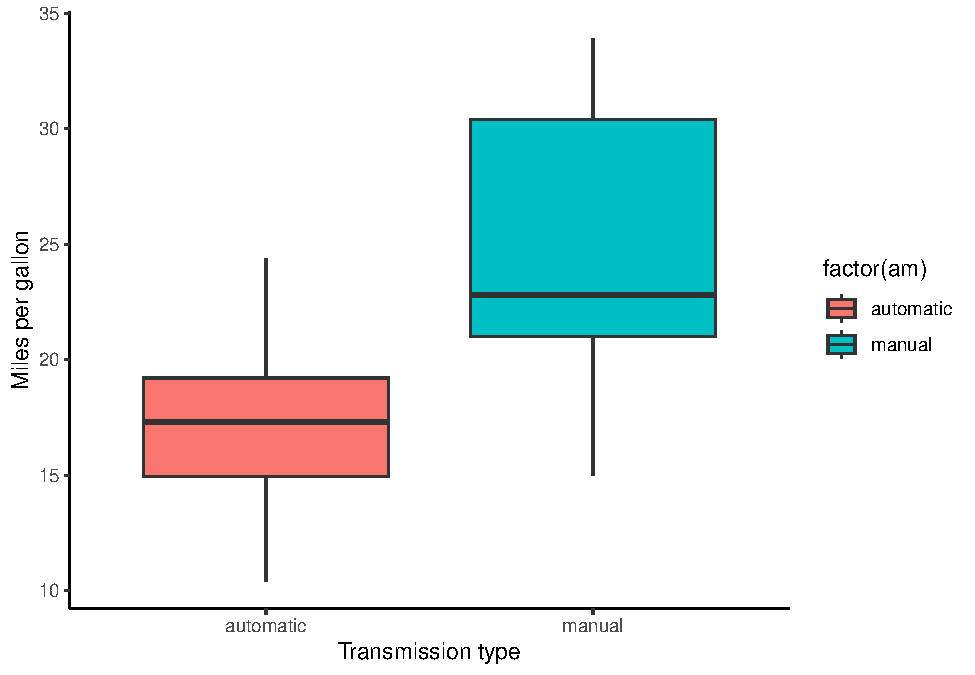
\includegraphics{Regression-Model-Course-Assignment_files/figure-latex/unnamed-chunk-20-1.pdf}

\subsection{Regression diagnostics
plot}\label{regression-diagnostics-plot}

\begin{Shaded}
\begin{Highlighting}[]
\FunctionTok{par}\NormalTok{(}\AttributeTok{mfrow =} \FunctionTok{c}\NormalTok{(}\DecValTok{2}\NormalTok{, }\DecValTok{2}\NormalTok{))}
\FunctionTok{plot}\NormalTok{(bestModel)}
\end{Highlighting}
\end{Shaded}

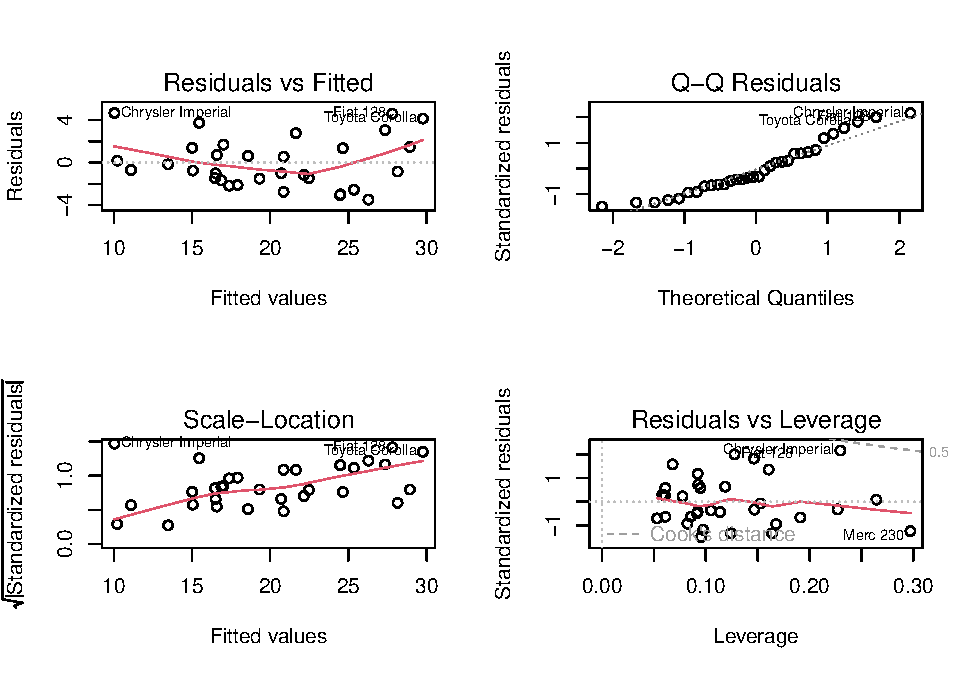
\includegraphics{Regression-Model-Course-Assignment_files/figure-latex/unnamed-chunk-21-1.pdf}

\subsection{Session info}\label{session-info}

\begin{Shaded}
\begin{Highlighting}[]
\FunctionTok{sessionInfo}\NormalTok{()}
\end{Highlighting}
\end{Shaded}

\begin{verbatim}
## R version 4.3.2 (2023-10-31 ucrt)
## Platform: x86_64-w64-mingw32/x64 (64-bit)
## Running under: Windows 11 x64 (build 22631)
## 
## Matrix products: default
## 
## 
## locale:
## [1] LC_COLLATE=English_India.utf8  LC_CTYPE=English_India.utf8   
## [3] LC_MONETARY=English_India.utf8 LC_NUMERIC=C                  
## [5] LC_TIME=English_India.utf8    
## 
## time zone: Asia/Calcutta
## tzcode source: internal
## 
## attached base packages:
## [1] stats     graphics  grDevices utils     datasets  methods   base     
## 
## other attached packages:
## [1] kableExtra_1.4.0 pander_0.6.5     printr_0.3       broom_1.0.5     
## [5] car_3.1-2        carData_3.0-5    dplyr_1.1.4      GGally_2.2.1    
## [9] ggplot2_3.5.1   
## 
## loaded via a namespace (and not attached):
##  [1] utf8_1.2.4         generics_0.1.3     tidyr_1.3.1        xml2_1.3.6        
##  [5] stringi_1.8.3      digest_0.6.34      magrittr_2.0.3     evaluate_0.23     
##  [9] grid_4.3.2         RColorBrewer_1.1-3 fastmap_1.1.1      plyr_1.8.9        
## [13] backports_1.4.1    purrr_1.0.2        fansi_1.0.6        viridisLite_0.4.2 
## [17] scales_1.3.0       abind_1.4-5        cli_3.6.2          rlang_1.1.3       
## [21] munsell_0.5.0      withr_3.0.0        yaml_2.3.8         tools_4.3.2       
## [25] colorspace_2.1-0   ggstats_0.7.0      vctrs_0.6.5        R6_2.5.1          
## [29] lifecycle_1.0.4    stringr_1.5.1      pkgconfig_2.0.3    pillar_1.9.0      
## [33] gtable_0.3.4       glue_1.7.0         Rcpp_1.0.12        systemfonts_1.1.0 
## [37] highr_0.10         xfun_0.49          tibble_3.2.1       tidyselect_1.2.1  
## [41] rstudioapi_0.15.0  knitr_1.45         farver_2.1.1       htmltools_0.5.7   
## [45] rmarkdown_2.26     svglite_2.1.3      labeling_0.4.3     compiler_4.3.2
\end{verbatim}

\end{document}
